\documentclass[
    11pt,
    a4paper,
    egregdoesnotlikesansseriftitles,
    toc=chapterentrywithdots,
    twoside,openright,
    titlepage,
    parskip=half,
    headings=normal,  % reduces heading size
    listof=totoc,
    bibliography=totoc,
    index=totoc,
    captions=tableheading,  % caption below table
    chapterprefix,
    listof=flat,
    final
]{scrbook}



% details about your thesis
\newcommand{\titel}{Automatisierte Provisionierungsmechanismen für Laufzeitumgebungen von Legacy z/OS Anwendungen mit „IBM Cloud Provisioning and Management for z/OS“ am Beispiel der „Rechnungsschreibung“ bei DATEV eG}
\newcommand{\artderarbeit}{Bachelorarbeit}  % {Bachelorarbeit,Masterarbeit}
\newcommand{\autor}{David Krug}
\newcommand{\studiengang}{Informatik}  % {Informatik,Wirtschaftsinformatik,Medieninformatik}
\newcommand{\matrikelnr}{3036355}
\newcommand{\erstgutachter}{Prof.\,Dr.~Korbinian Riedhammer}
\newcommand{\zweitgutachter}{Prof.\,Dr.~Friedhelm Stappert}
\newcommand{\logo}{figures/TH-Nuernberg-RGB.png}
\newcommand{\keywords}{hot, fuzz}
 


% custom head and foot
\usepackage[automark]{scrlayer-scrpage}
\pagestyle{scrheadings}
\ihead{\headmark}
\chead{}
\ohead{\pagemark}
\renewcommand*\chaptermarkformat{\chapappifchapterprefix{\ }% 
  \thechapter.\enskip}

\RedeclareSectionCommand[tocindent=0pt]{section}
\RedeclareSectionCommand[tocindent=0pt]{subsection}
%\RedeclareSectionCommand[tocnumwidth=70pt]{chapter}

\usepackage{scrhack}

% other packages
\usepackage[utf8]{inputenc}
\usepackage[T1]{fontenc}
\usepackage{lmodern,relsize,textcomp,csquotes}
\usepackage{amsmath,amsfonts}
\usepackage[ngerman]{babel}  % flip for German thesis
\usepackage[final]{graphicx}
\usepackage{setspace,geometry,xcolor}
\usepackage{makeidx}
\usepackage{paralist,ifthen,todonotes}
\usepackage{url}
\usepackage{pdfpages}

% table setup
\usepackage{longtable}
\usepackage{array}
\usepackage{ragged2e}
\usepackage{lscape}

% pdf hyperref
\usepackage[
    bookmarks=true,
    bookmarksopen=true,
    bookmarksnumbered=true,
    bookmarksopenlevel=1,
    pdftitle={\titel},
    pdfauthor={\autor},
    pdfcreator={\autor},
    pdfsubject={\titel},
    pdfkeywords={\keywords},
    pdfpagelabels=true,
    colorlinks=true,
    linkcolor=red,
    urlcolor=magenta,
    anchorcolor=black,
    citecolor=cyan,
    filecolor=magenta,
    menucolor=red,
    plainpages=false,
    hypertexnames=true,
    linktocpage=true,
]{hyperref}


% configure your listings style
\usepackage{listings}
\lstset{
	tabsize=3,
	extendedchars=true,
	frame=single,
	showstringspaces=true,
	numbers=left,
	numberstyle=\small,
	breakautoindent=true
}

% page setup
% \setlength{\topskip}{\ht\strutbox}
\geometry{paper=a4paper,left=2.5cm,top=3.0cm,bindingoffset=.8cm}
\onehalfspacing
\frenchspacing
\clubpenalty = 10000
\widowpenalty = 10000 
\displaywidowpenalty = 10000

% some commands
\newcommand{\ua}{\mbox{u.\,a.\ }}
\newcommand{\zB}{\mbox{z.\,B.\ }}
\newcommand{\dahe}{\mbox{d.\,h.,\ }}
\newcommand{\bzw}{\mbox{bzw.\ }}
\newcommand{\bzgl}{\mbox{bzgl.\ }}
\newcommand{\eg}{\mbox{e.\,g.\ }}
\newcommand{\ie}{\mbox{i.\,e.\ }}
\newcommand{\wrt}{\mbox{w.\,r.\,t.\ }}
\newcommand{\etal}{\mbox{\emph{et.\,al.\ }}}
\renewcommand*\contentsname{Inhaltsverzeichnis}


% TODO remove if not needed...
\usepackage{blindtext}


\begin{document}

\setcounter{secnumdepth}{3}  % numerate subsections
\setcounter{tocdepth}{2}  % ...but don't include them in toc

\frontmatter
\include{cover}\cleardoublepage

% download the following form and complete it (hit save in your editor)
% https://intern.ohmportal.de/fileadmin/Gelenkte_Doks/Abt/SZS/SB/SB_0050_FO_Pruefungsrechtliche_Erklaerung_und_Erklaerung_zur_Veroeffentlichung_der_Abschlussarbeit_public.pdf
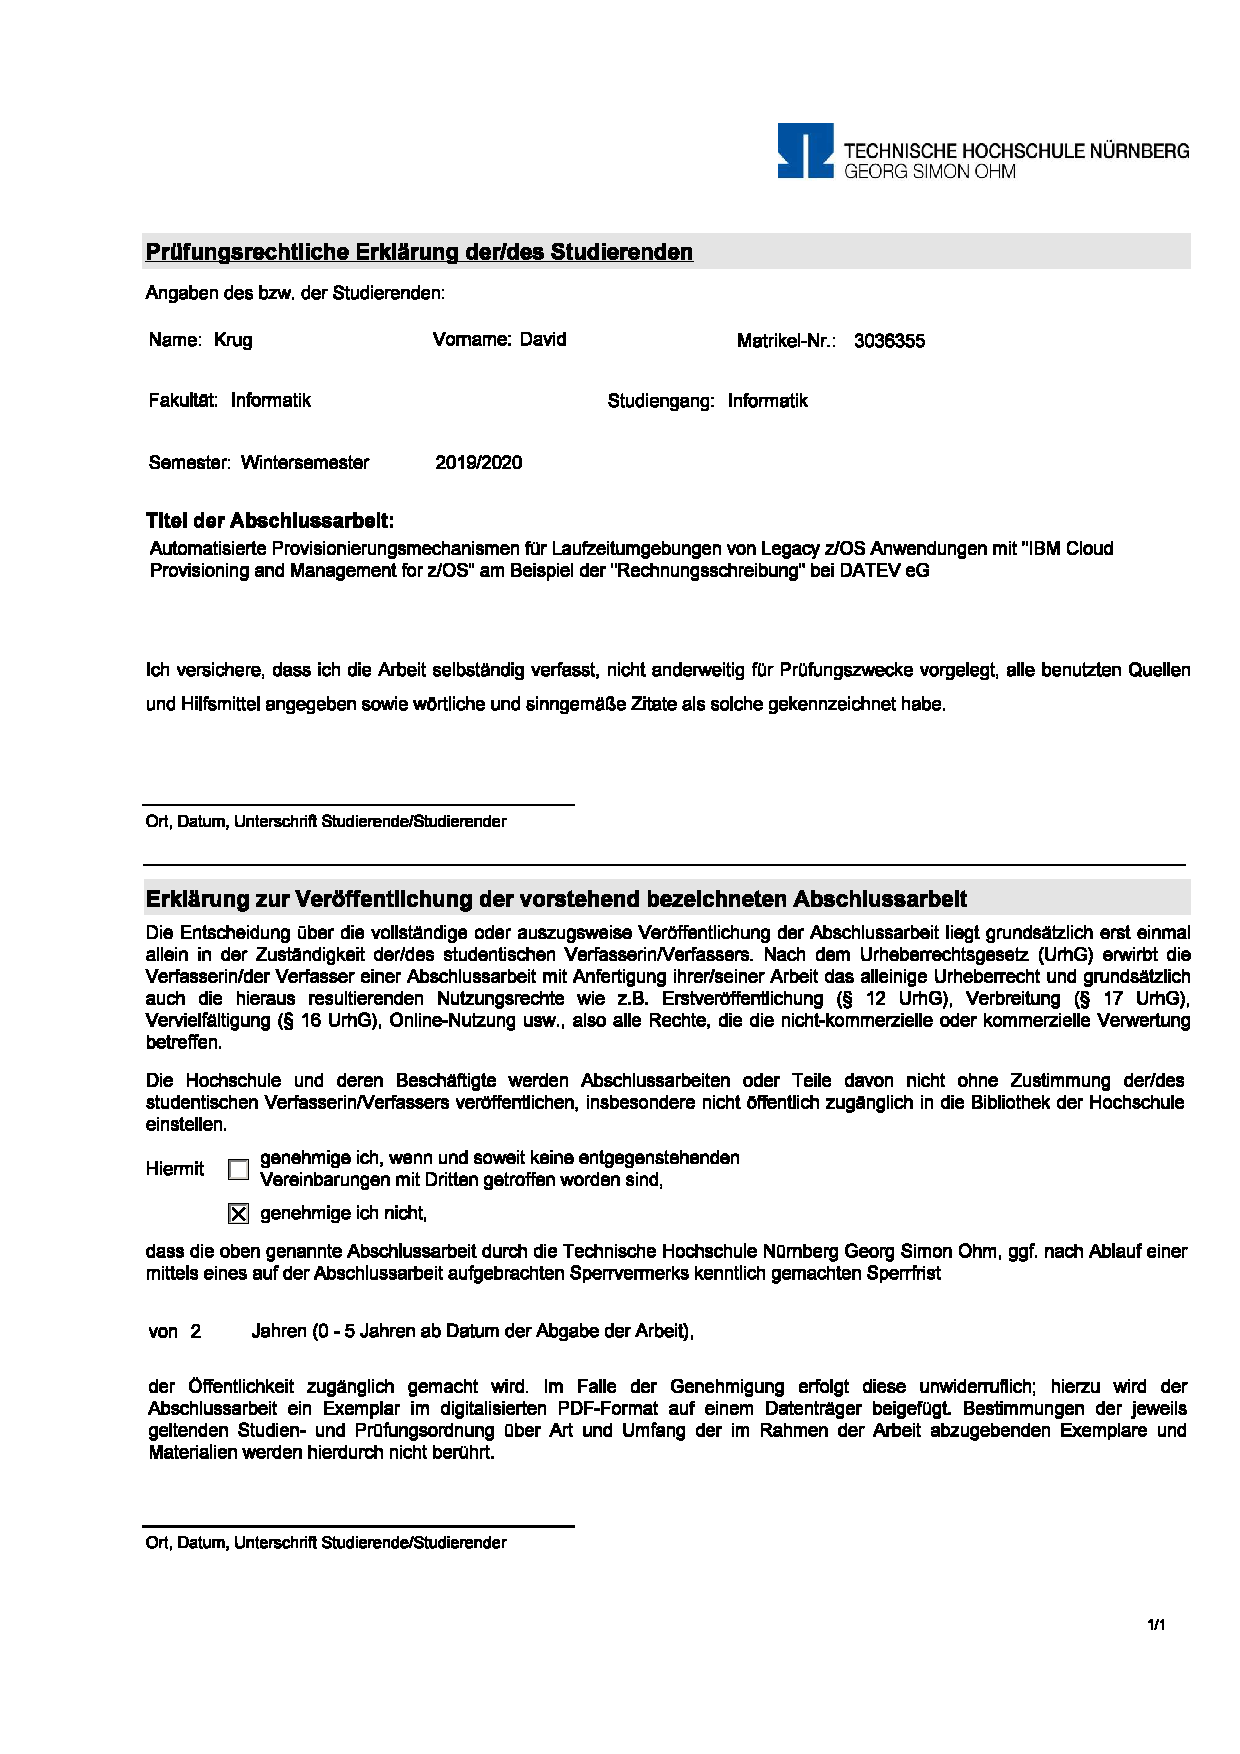
\includepdf{SB_0050_FO_Pruefungsrechtliche_Erklaerung_und_Erklaerung_zur_Veroeffentlichung_der_Abschlussarbeit_public.pdf}\cleardoublepage

\thispagestyle{empty}
\section*{Kurzdarstellung}
\label{sec:kurzdarstellung}
Ziel dieser Arbeit ist es, zu bestimmen, ob die Bereitstellung von Laufzeitumgebungen für legacy z/OS Anwendungen über einen cloud nativen, Platform-as-a-Service Ansatz bei DATEV e.G. möglich ist.
Es werden folgende Forschungsfragen gestellt:
\begin{itemize}
\item Ist es möglich, den Bereitstellungsprozess für z/OS Anwendung bei DATEV e.G. mit Hilfe des \glqq IBM Cloud Provisioning and Management for z/OS\grqq-Tools an cloud native Prozesse ("Self Service") anzunähern?
\item Erzeugt die Nutzung von \glqq IBM Cloud Provisioning and Management for z/OS\grqq{} einen Mehrwert bei den Stakeholdern, also den Entwicklerteams und den Administratorenteams?
\end{itemize}

Dafür wurde anhand einer Beispielanwendung von DATEV das Tool \glqq IBM Cloud Provisioning and Management for z/OS\grqq untersucht.
Es wurden zwei vorhandene Möglichkeiten aufgezeigt, eine davon implementiert.
Für ein Meinungsbild bezüglich  Mehrwertes und Akzeptanz des Tools, wurden Interviews mit Stakeholdern durchgeführt.
Diese Bild zeigt, dass in dem Tool eine Chance auf Verbesserung der aktuellen Prozesse gesehen wird.

Ergebnis war auch, dass die implementierte Variante nicht optimal für den Praxiseinsatz bei DATEV e.G. ist, aber eine wichtige Basis für die automatisierte Bereitstellung von Laufzeitumgebungen für z/OS Anwendungen darstellt.
Weiterführende Forschung könnte darauf aufbauend Variante zwei untersuchen und  Möglichkeiten einer weiteren, parxisgeeigneteren  Optimierung des z/OS Bereitstellungsprozesses aufzeigen.



\cleardoublepage

\tableofcontents

\mainmatter
\chapter{Einführung}\label{ch:intro}

You may have read about similar things in \cite{Goodliffe2007}.
You can also write footnotes.\footnote{Footnotes will be positioned automatically.}
\blindtext

\blindtext

\section{This is an Important Section}
\blindtext

\subsection{And an even more important subsection}
\blindtext

\chapter{Grundlagen}\label{ch:data}

\Blindtext

\chapter{Vorgehensweise}\label{ch:method}

In this chapter, we're actually using some code!

\begin{lstlisting}[language=Python,caption={This is an example of inline listing},captionpos=b]
x = 1
if x == 1:
    # indented four spaces
    print("x is 1.")

\end{lstlisting}

You can also include listings from a file directly:

\lstinputlisting[language=Python,caption={This is an example of included listing},captionpos=b]{listings/example.py}

\include{content/4_experiments}
\include{content/5_outlook}
\include{content/6_summary}

% remove if not needed
\appendix
\include{content/a1_supplemental}

\backmatter
\listoffigures
\cleardoublepage

\listoftables
\cleardoublepage

\renewcommand{\lstlistlistingname}{Quellcodeverzeichnis}  % change for German thesis
\renewcommand{\lstlistingname}{Quellcode}
\lstlistoflistings
\cleardoublepage

\bibliographystyle{wmaainf}
\bibliography{refs}

\end{document}
